\section{Методика~использования программного средства}
\label{sec:usage}

\subsection{Руководство по установке и настройке}

На компьютере-сервере для корректной установки серверной части должно быть установлено следующее программное обеспечение:
\begin{itemize}
	\item операционная система семейства Windows или Linux; 
	\item Java версии не ниже 1.7;
	\item MySQL сервер версии начиная с 5.1;
	\item веб-сервер apache tomcat.
\end{itemize}

Порядок установки серверной части:
\begin{itemize}
	\item скачиваем последнию версию Java; 
	\item распаковываем архив на диске;
	\item Необходимо прописать путь до файлов JDK в путях операционной системы. Это позволит запускать основные файлы из командной строки. В переменых среды необходимо создать JAVAHOME и прописать путь до папки с JDK. После этого необходимо добавить переменую JAVAHOME в переменую PATH;
	\item скачиваем последнию версию apache tomcat;
	\item распаковываем архив на диске;
	\item скопировать файл SocialNetWork.war в папку tomcat/webapps;
	\item скачать и установить последнию версию Mysql сервер;
	\item необходимо сделать импорт базы данных. Открываем консоль и прописываем следующую команду "mysql -u username -p databaseТame < socialNetwork.sql";
	\item следующим пунктом необходимо запусть apache tomcat. Переходим в tomcat/bin. Необходимо выполнить в консоль catalina.bat run; 
\end{itemize}

Порядок установки клиетской части:
\begin{itemize}
	\item скачиваем последнию версию Node js; 
	\item распаковываем архив на диске;
	\item переходим в tomcat/webapps/SocialNetWork;
	\item слудующим пунктов необходимо выполнить команду "npm run server";
\end{itemize}

После установления всех настроек в браузере должна отобразиться страница, означающая, что серверная часть установлена корректно.

\subsection{Руководство по использованию}

Внешний вид программного средства сразу после запуска представлен на рисунке \ref{fig:sec_usage::home_page}. Как видно из представленного рисунка, всю область, которую занимает программное средство можно условно поделить на три следующие части: 

\begin{itemize}
	\item главная страница; 
	\item регистрация пользователь;
	\item вход в приложение;
\end{itemize}

Главная страница предоставляет краткое описание основных возможностей программного средства для пользователей. Страница регистрации позволяет создать новую учетную запись, чтобы использовать программное средство для работы. Страница входа в приложения служит точкой начала использования программного срдества. 

\begin{figure}[!htb]
	\centering
	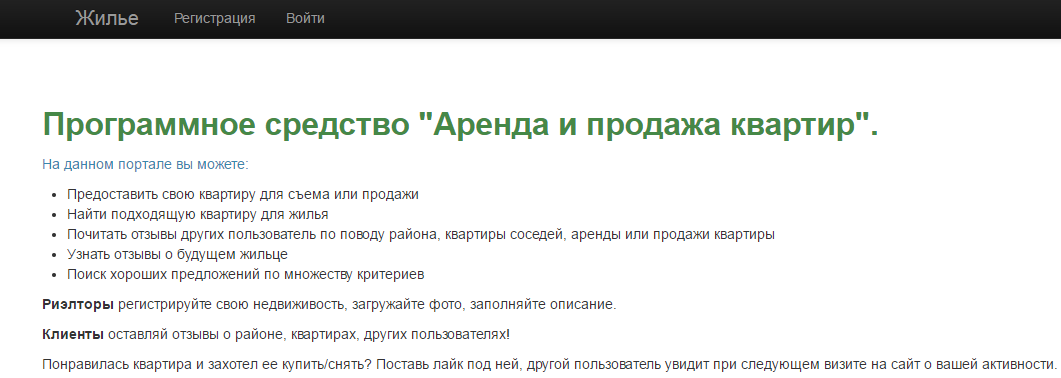
\includegraphics[scale=0.586]{home_page.png}
	\caption{ Внешний вид программного средства }
	\label{fig:sec_usage::home_page}
\end{figure}

На рисунке \ref{fig:sec_usage::reg} представлена страница, для создания учетной записи пользователя. Для создания новой учетной записи необходимо указать следующие обязательные поля: 

\begin{itemize}
	\item Логин. Данная информация будет использоватся в качестве входа в программное средство; 
	\item Пароль. Данная информация будет использоватся в качестве входа в программное средство;
	\item Электронная почта. Данная информация будет использоватся для восстановления пароля;
	\item Фамилия. Данная информация будет отображена для других пользователей программного средства;
	\item Имя. Данная информация будет отображена для других пользователей программного средства;
	\item Телефон. Данная информация будет использоватся в качестве взаимодействия с другими пользователями;
	\item Город. Данная информация нужна для поиска;
	\item Роль пользователя. Исходя из этой информации, будущему пользователю будут доступны необходимые функции приложения;
\end{itemize}

\begin{figure}[!htb]
	\centering
	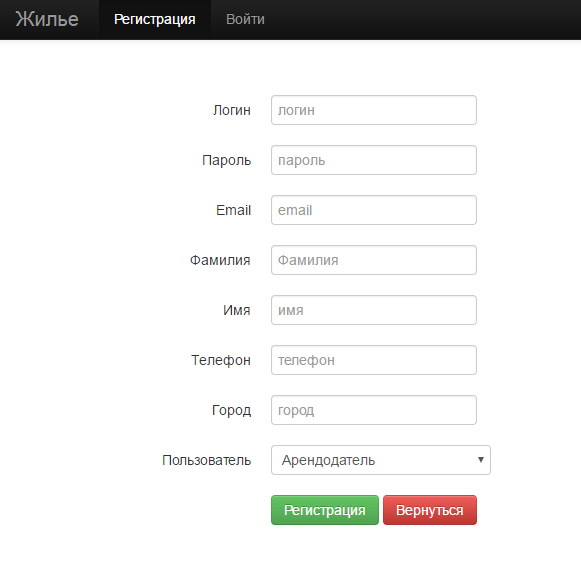
\includegraphics[scale=1]{registration.png}
	\caption{ Форма для создания нового пользователя }
	\label{fig:sec_usage::reg}
\end{figure}

На рисунке \ref{fig:sec_usage::signIn} представлена страница, для входя в программное средство. Для входа необходимо указать обязательные поля:

\begin{itemize}
	\item Логин; 
	\item Пароль;
\end{itemize}

Помимо этого на данной форме есть функция для восстановления пароля, в случае, если пользователь забыл пароль от своей учетной записи. Чтобы восстановить пароль, необходимо указать электронную почту, которая была указана при регистрации.

\begin{figure}[!htb]
	\centering
	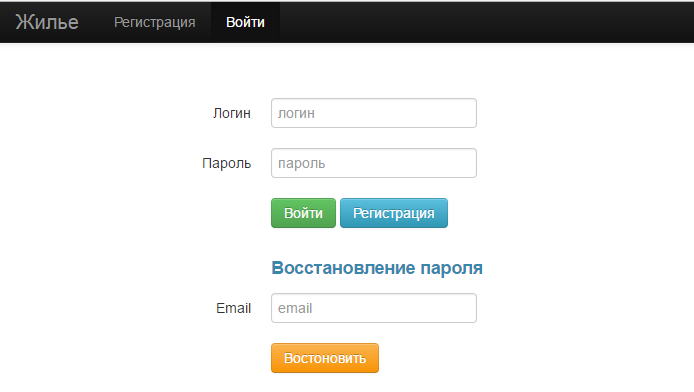
\includegraphics[scale=0.9]{signIn.png}
	\caption{ Форма для восстановления пароля и входа в программное средство}
	\label{fig:sec_usage::signIn}
\end{figure}

После входа в приложения, пользователь увидит главный экран своей страницы. На нем отображены информация при регистрации. Помимо этого, можно посмотреть отзывы о себе, перейти на страницу поиска, изменить информацию о себе.

Для изменения информации, необходимо перейти в раздел настройки. Чтобы это сделать, нужно нажать на кнопку настройку. Для каждого из пользователь, страница выглядит с отличиями. Рассмотрим случай, когда пользователь продает свою квартиру. В разделе настройки, необходимо заполнить цену продажи/аренды. Добавить краткое описание. Помимо этого можно загрузить изображения будущей квартиры. 

Чтобы загрузить изображения для своей недвижимости, необходимо перейти в раздел настройки. Далее нажимаем кнопку загрузить фотографии. В появившемся окошке выбираем фотографии, которые находятся на жестком диске, и нажимаем загрузить. После того, как изображения будут загружены, пользователь смотрит их посмотреть в своем профиле.

Рассмотрим пользователя, который хочет купить недвижимость. Для поиска необходимой недвижимости, необходимо перейти в раздел поиска. На главной форме нажимаем кнопку поиск предложений. После этого будет отображена страница для поиска предложений. На данном этапе можно использовать множество критериев, которые необходимы конечному пользователю. 
   

\begin{figure}[!htb]
	\centering
	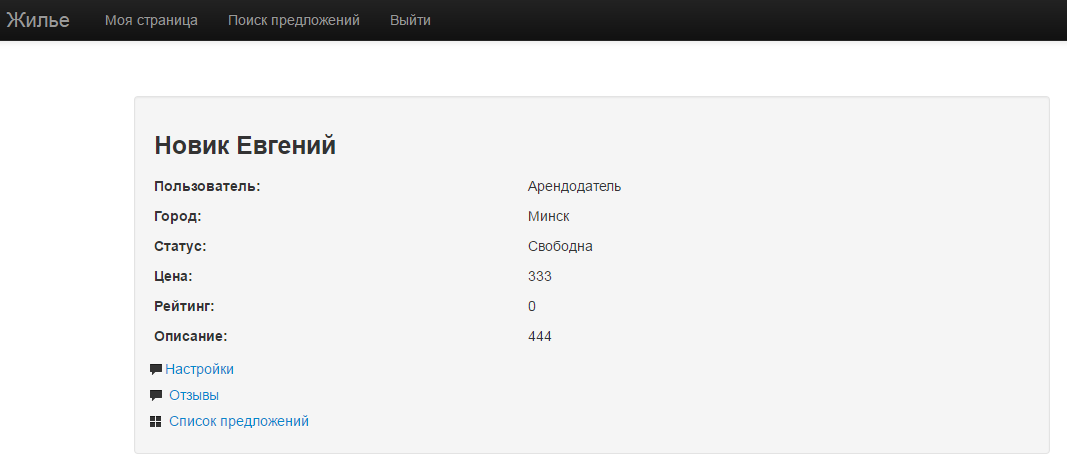
\includegraphics[scale=0.5]{b_settings.png}
	\caption{ Страница после входа в приложение}
	\label{fig:sec_usage::signIn}
\end{figure}

\begin{figure}[!htb]
	\centering
	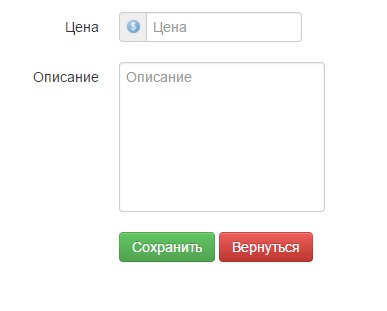
\includegraphics[scale=0.9]{settings.png}
	\caption{ Страница редактирования квартиры}
	\label{fig:sec_usage::signIn}
\end{figure}

После заполнений необходимых полей поиска, нажимаем на кнопку найти. После поиска, на странице появятся перечень квартир, которые можно купить/арендовать. Если пользователю понравилась квартира, ему достаточно нажать на кнопку "Нравится". Хозяину квартиры придет уведомление, что квартирой интересуется другой пользователь. У пользователей будет видна информация, для связи друг с другом, после двухэтапная аутентификации. 

\begin{figure}[!htb]
	\centering
	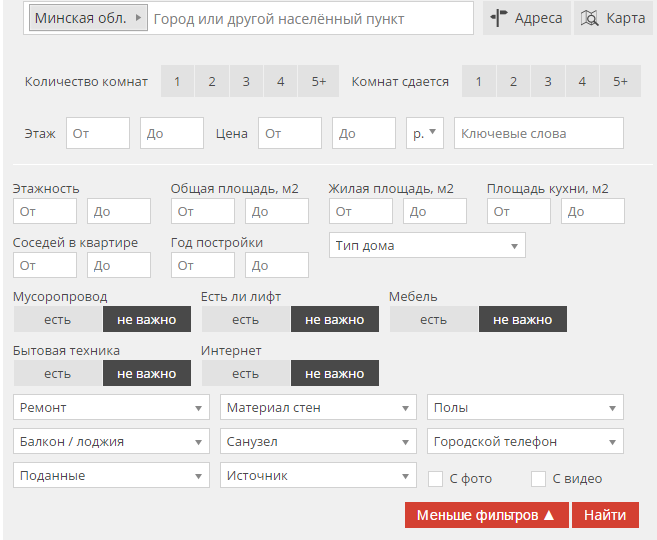
\includegraphics[scale=0.9]{search.png}
	\caption{ Страница поиска квартир}
	\label{fig:sec_usage::signIn}
\end{figure}

Чтобы просмотреть отзывы об недвижимости, которую сдают в аренду, необходимо перейти на квартиру и нажать на кнопку отзывы.

На данной странице отображены отзывы других пользователей. Здесь можно узнать мнение другого человека. Отзыв состоит из текста, времени и даты, когда он был создан.

\clearpage

